\documentclass{article}
\usepackage[utf8]{inputenc}
\usepackage[T1]{fontenc}
\usepackage[portuguese]{babel}

\usepackage{indentfirst}
\usepackage{makeidx}
\usepackage{stackengine}
\usepackage{amssymb}
\usepackage{amsthm}
\usepackage{hyperref}
\usepackage{color}
\usepackage{graphicx}

\usepackage{pdfpages}
\usepackage{float}

\usepackage{booktabs}

\usepackage[showframe=false]{geometry}
\usepackage{changepage}


\title{\bf{Aprendizagem Computacional - Trabalho Prático 4}\vspace{80mm}}
\author{\textbf{João Tiago Márcia do Nascimento Fernandes - 2011162899} \\
\textbf{Joaquim Pedro Bento Gonçalves Pratas Leitão - 2011150072}}
\makeindex

\begin{document}

\maketitle

\pagebreak

\renewcommand*\contentsname{Índice}
\tableofcontents

\pagebreak

\section{Introdução}

O presente trabalho visa a implementação de controladores difusos de um dado sistema, dos tipos \emph{Mamdani} e \emph{Sugeno}, e que representam um hipotético processo real, tendo como base do seu funcionamento regras da \emph{lógica difusa}.

A \emph{lógica difusa} extende o conceito de \emph{lógica booleana}, admitindo valores lógicos intermediários entre os valores de \emph{FALSO} e \emph{VERDADEIRO}. Assim, a lógica difusa permite-nos extender o conceito de conjunto, permitindo que um elemento passe a possuir um \emph{grau de pertença} num dado conjunto, cujo valor varia entre \emph{0} e \emph{1}.

Um controlador que se rege por essa lógica, ou seja, um \emph{controlador difuso}, possuí um conjunto de regras lógicas, e é constituído por três fases:

\begin{itemize}
\item \emph{Fase entrada}
\item \emph{Fase de processamento}
\item \emph{Fase de saída}
\end{itemize}

A fase de entrada mapeia a entrada recebida pelo controlador nas funções de pertença e valores de verdade apropriados. Já na fase de processamento, as regras lógicas apropriadas à entrada recebida são invocadas, combinando o seu resultado, que é devolvido na fase de saída, sendo codificado num valor específico.

Relativamente aos controladores disponíveis na aplicação, estes foram desenvolvidos no ambiente \emph{Simulink}, em conjunto com a \emph{Fuzzy Logic Toolbox}, ambos pertencentes à plataforma \emph{Matlab}. Numa fase inicial do trabalho apenas foram desenvolvidos controladores de $9$ regras, tendo esse valor aumentado para $25$ numa fase posterior do trabalho.

No presente documento pretendemos apresentar de forma mais detalhada os controladores implementados, discutindo alguns detalhes relativos à sua implementação e apresentando uma reflexão crítica sobre o desempenho e performance dos diferentes controladores implementados (\emph{Mamdani} e \emph{Sugeno}, de \emph{9} e \emph{25} regras).


\pagebreak

\section{Aplicação Desenvolvida}

A aplicação desenvolvida visa implementar os controladores difusos referidos anteriormente, representando um hipotético processo real, cujo funcionamento pode ser simulado, através da aplicação.

Para isso, a aplicação foi implementada em \emph{Matlab}, recorrendo à \emph{Fuzzy Logic Toolbox} do \emph{Simulink}, de forma a permitir a simulação do processo.

A aplicação faz ainda uso de uma interface por linha de comandos (\emph{CLI - Command Line Interface}), que permite ao utilizador escolher as características do processo que pretende simular: tipo de controlador, número de regras e tipos de perturbações, referência, entre outros.

\subsection{Processo}

Para a aplicação em questão, foram atribuídos a cada grupo diferentes processos a simular, sendo que cada processo é caracterizado por uma função de transferência diferente.

O processo que nos foi atribuído é caracterizado pela seguinte função de transferência:

$$\frac{3\times (s + 1)}{s\times (s + 2)\times (s + 4)}$$


\subsection{Referências}

Nesta aplicação encontram-se disponíveis dois tipos diferentes de referências: Uma correspondente à \emph{onda quadrada}, e outra a uma \emph{onda senoide (seno)}, ambas de amplitude $1$.

Como podemos observar nas figuras seguintes, a onda senoide apresenta-se como a mais suave das duas ondas, contendo variações menos pronunciadas, quando comparada com a onda quadrada.

\begin{figure}[H]
  \centering
      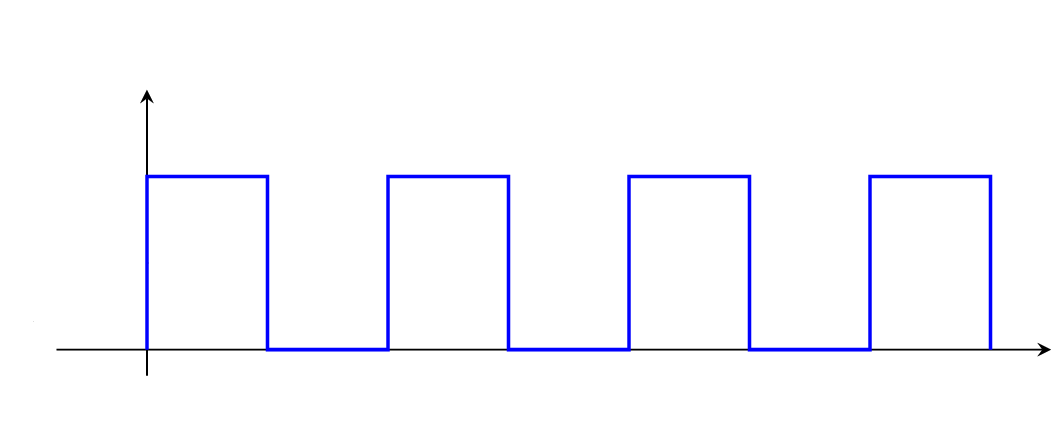
\includegraphics[scale=0.3]{Images/Squared_Wave.png}
  \caption{Exemplo de uma onda quadrada}
\end{figure}

\begin{figure}[H]
  \centering
      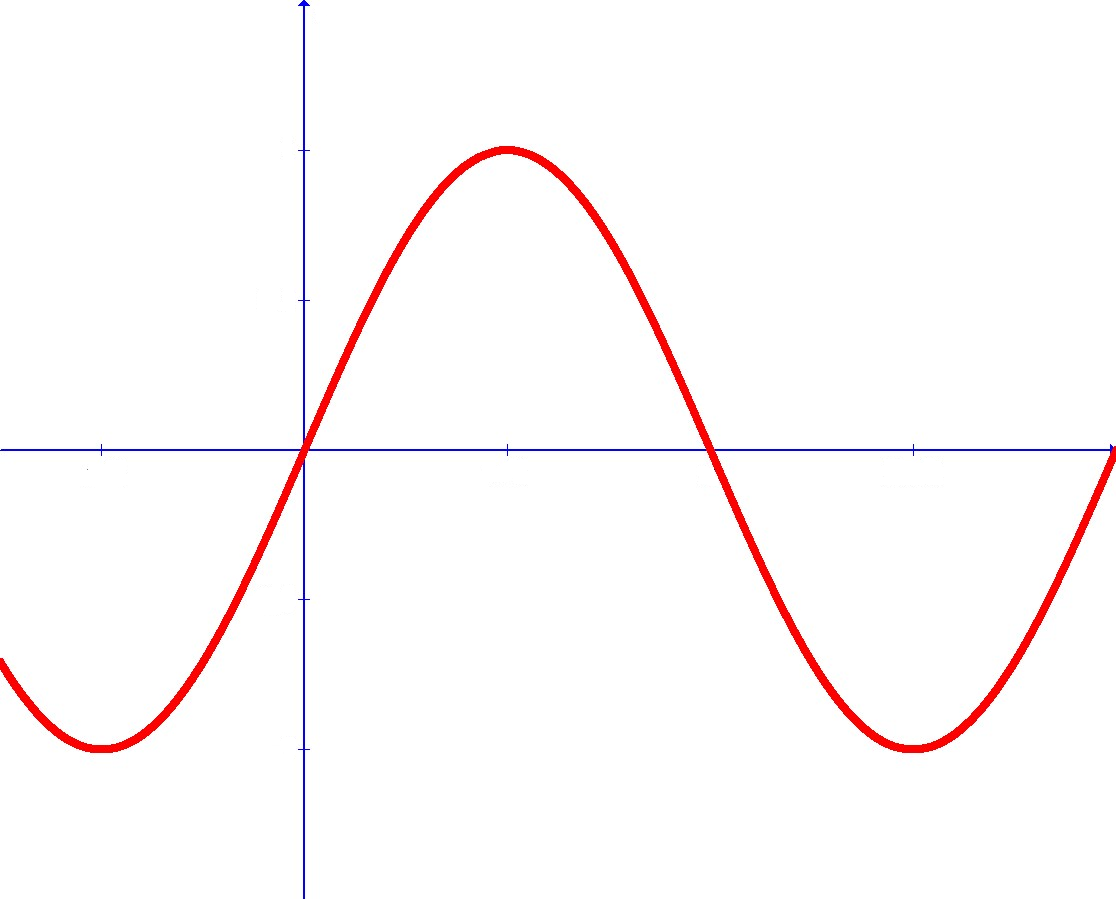
\includegraphics[scale=0.2]{Images/Sin_Wave.png}
  \caption{Exemplo de uma onda senoide}
\end{figure}

Esta última é caracterizada por períodos em que o seu valor se mantém constante, que alternam com pontuais momentos onde esta muda bruscamente o seu valor.

Estas constantes e abruptas variações têm um efeito negativo no controlador, resultando em erros mais pronunciados, e numa performance superior (o que na presente situação, em que a performance é medida em função o integral do erro quadrático, não é uma situação de todo desejada).

Assim, será de prever melhores desempenhos quando a referência fornecida ao controlador é a onda senoide, do que quando este tem como referência uma onda quadrada.


\subsection{Controladores}

Relativamente aos \emph{controladores} implementados, encontram-se disponíveis dois tipos distintos: Controladores \emph{Mamdani} e \emph{Sugeno}, ambos com implementações de $9$ e $25$ regras.

Efetivamente, ao variarmos o número de regras em cada controlador estamos a alterar a ação por ele tomada, uma vez que o valor à saída do controlador está dependente da aplicação dessas regras lógicas à sua entrada.

Mais ainda, se aumentarmos o número de regras do controlador, mantendo todas as outras características constantes, seria de esperar uma melhoria na sua performance, uma vez que com um maior número de regras os ajustes realizados pelo controlador podem ser mais suaves e adaptados a cada situação em particular.

Assim, quanto menor for o número de regas, maior terá que ser a generalização de cada regra, culminando num maior erro do controlador, e numa performance inferior.

Nas figuras que se seguem apresentamos as tabelas com as regras implementadas nos controladores, onde:

\begin{itemize}
\item N - Negativo
\item ZE - Zero
\item P - Positivo
\item NB - Negativo Grande
\item NS - Negativo Pequeno
\item PS - Positivo Pequeno
\item PB - Positivo Grande
\end{itemize}


\begin{figure}[H]
  \centering
      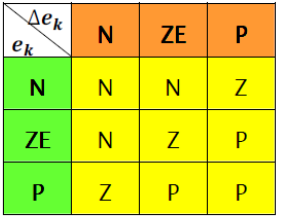
\includegraphics[scale=0.5]{Images/9_Rules.png}
  \caption{Tabela com as 9 regras implementadas por um controlador de 9 regras}
\end{figure}

\begin{figure}[H]
  \centering
      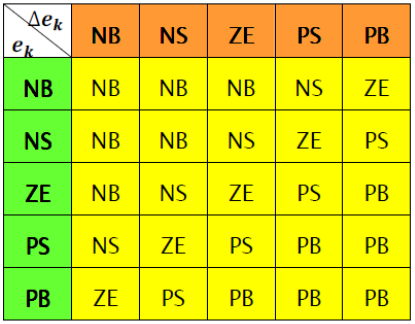
\includegraphics[scale=0.5]{Images/25_Rules.png}
  \caption{Tabela com as 25 regras implementadas por um controlador de 25 regras}
\end{figure}

Desta forma, implementámos controladores com as seguintes características:

\begin{itemize}
\item Tipo \emph{Mamdani} ou \emph{Sugeno}
\item Função de pertença do tipo \emph{trimf}
\item Operadores \emph{min-max}
\item Desfuzificação do tipo \emph{Centróide}
\end{itemize}

Efetivamente, gostaríamos de apresentar neste trabalho mais variações nas características dos controladores, no entanto não dispusemos do tempo necessário para o fazer.


\subsection{Perturbações}

Numa primeira fase do trabalho, pretendemos estudar o desempenho dos diferentes controladores ao seguirem uma dada entrada, ignorando qualquer perturbação do sinal gerado. Posteriormente, surge com naturalidade o estudo do comportamento e desempenho dos mesmos controladores quando sujeitos a entradas de alguma forma adulteradas ou \emph{perturbadas}.

Assim, introduzimos perturbações nos sinais de referência gerados, que podem atuar ao nível dos \emph{atuadores} e/ou da \emph{carga} do controlador, com o objetivo de verificarmos como é que cada controlador compensa essas perturbações.

Uma vez que estamos a adulterar os sinais de entrada do controlador, facilmente prevemos que o seu desempenho diminuirá quando sujeito a entradas desta forma adulteradas. Mais ainda, quando estas ocorrem ao nível do atuador e da carga, em simultâneo, será de esperar que o controlador apresente desempenho inferior, do que quando as perturbações se dão apenas na carga ou no atuador. Isto deve-se ao facto de estas perturbações introduzirem variações na referência, que são, naturalmente, mais difíceis de seguir para o controlador.

Desta forma, no presente trabalho, incluímos os seguintes cenários relativos a existência de perturbações na referência do controlador:

\begin{itemize}
\item Ausência de perturbações na referência do controlador
\item Perturbações ao nível do atuador
\item Perturbações ao nível da carga
\item Perturbações ao nível do atuador e da carga
\end{itemize}


\subsection{Implementação}

Tal como referimos no início do documento, a aplicação foi desenvolvida em \emph{Matlab}, recorrendo ao seu ambiente de simulação, o \emph{Simulink} e à sua biblioteca de lógica difusa: \emph{Fuzzy Logic Toolbox}.

Assim, a nossa implementação consiste num pequeno ficheiro \emph{Matlab} (a partir do qual a aplicação é iniciada, e onde são selecionados os seus parâmetros), e num conjunto dos controladores implementados e dos modelos de simulação do processo.

Estes últimos, permitem-nos implementar o sistema a simular, possibilitando-nos a sua execução de acordo com os parâmetros especificados. Na figura seguinte apresentamos um exemplo de um modelo implementado:

\begin{figure}[H]
  \centering
      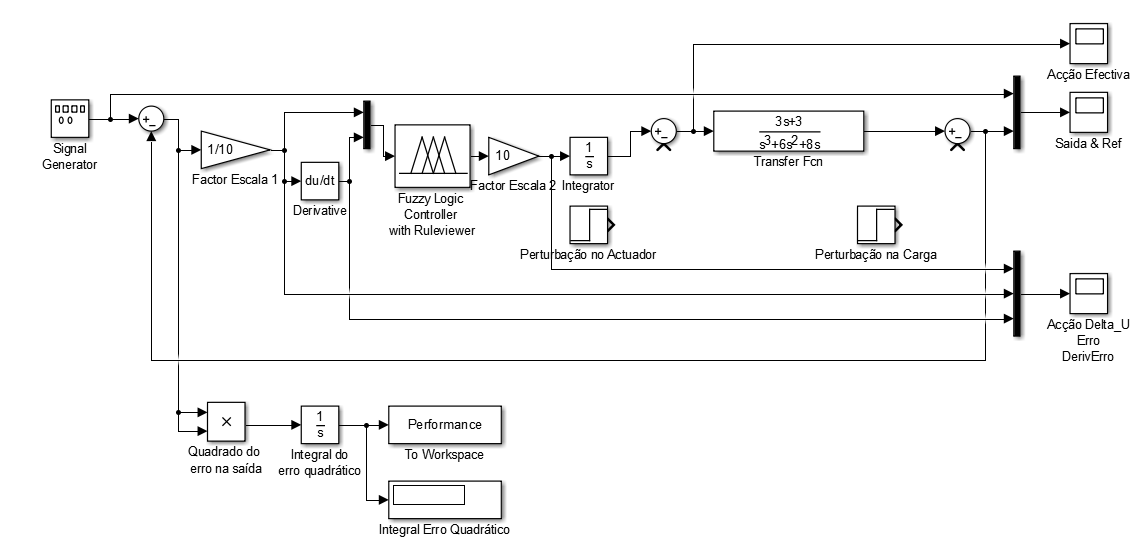
\includegraphics[scale=0.5]{Images/Controller_example.png}
  \caption{Exemplo de um modelo implementado em \emph{Simulink}}
\end{figure}

O modelo em questão pretende simular a existência de um controlador do tipo \emph{Mamdani} com $9$ regras (embora fosse possível considerar outro controlador, sem necessitar de proceder a alterações significativas no modelo), possuindo uma referência quadrada (à semelhança do controlador, poderíamos considerar outra referência sem necessitarmos de proceder a alterações significativas no modelo) e com ausência de perturbações.

Assim, implementámos um modelo diferente para cada situação a simular, tendo em conta o controlador a adotar, referência e perturbações a considerar.

\subsubsection{Modelos}

No que respeita à implementação dos modelos existe um aspeto relevante que, desde já, gostaríamos de salientar. Este aspeto prende-se com os fatores de escala e com a sua determinação.

Uma vez que não possuímos nenhum método analítico para determinar os fatores de escala que nos permitem obter os melhores resultados, a determinação dos fatores de escala a considerar foi realizada por \emph{tentativa-erro}, até encontrarmos um par de valores que nos permitissem obter resultados aceitáveis (ou o mais próximo disso possível) nos diferentes cenários considerados.

Após alguns testes, optámos por utilizar um fator de escala de $0.1$ à entrada do controlador, e um fator de escala de $10$ à saída do controlador. No entanto, acreditamos ser possível a utilização de outros fatores de escala que nos permitam obter melhores resultados.

\subsubsection{run.m}

Este ficheiro contém um \emph{script} que permite executar a aplicação. Neste \emph{script} o utilizador poderá definir todas as propriedades do sistema a simular. O funcionamento da aplicação, tal como a estrutura deste ficheiro, serão abordados em maior detalhe na secção que se segue.


\subsection{Execução}

Para executar a aplicação o utilizador deverá executar o ficheiro \emph{run.m}. Uma vez iniciada a execução, o utilizador deverá especificar as propriedades do sistema a simular, tais como:

\begin{itemize}
\item Referência do sistema (Onda senoide ou quadrada)
\item Tipo de controlador a implementar (Mamdani ou Sugeno)
\item Número de regras a implementar no controlador ($9$ ou $25$ regras)
\item Perturbações a considerar (Ausência de perturbações, perturbações no atuador e/ou na carga)
\end{itemize}

Uma vez definidas estas propriedades, será aberta uma janela contendo um modelo que representa o sistema escolhido (de acordo com as propriedades especificadas). O utilizador poderá executar este sistema clicando no botão de execução, presente na barra de opções no topo da janela.

Uma vez finda a execução do sistema, podemos consultar o seu desempenho consultando o campo \emph{IntegralErroQuadrático}, que, tal como o nome sugere, corresponde ao integral do erro quadrático (quadrado da diferença entre a saída do controlador e a referência considerada). Para visualizar a saída, basta clicar sobre o ícone com o nome \emph{Saída \& Ref}.

\pagebreak

\section{Testes da Aplicação}

Para podermos comparar o desempenho dos diferentes controladores implementados, nas situações consideradas, realizámos alguns testes à aplicação, que apresentamos de seguida.

\begin{figure}[H]
  \centering
      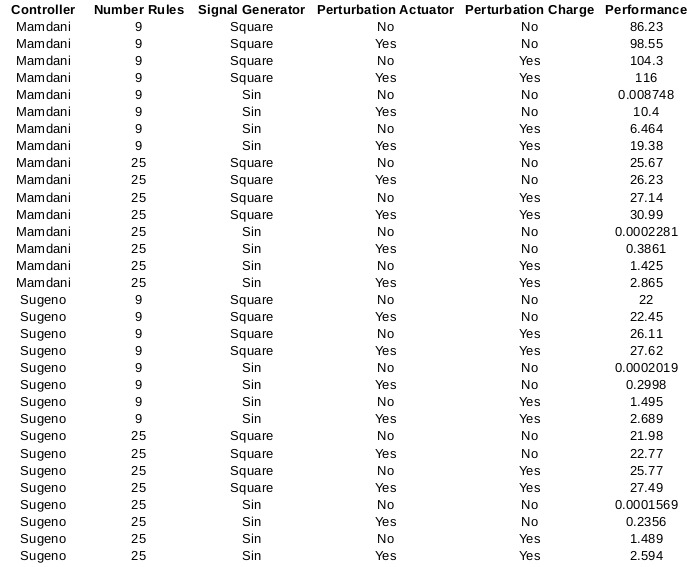
\includegraphics[scale=0.6]{Images/Results.png}
  \caption{Testes realizados}
\end{figure}

Para cada um dos controladores implementados testámos o seu desempenho para diferentes números de regras, referências e perturbações, mantendo todos os outros fatores iguais (nomeadamente os fatores de escala). Assim, testámos as seguintes configurações, para cada controlador:

\begin{itemize}
\item Considerar um total de $9$ e $25$ regras
\item Utilizar como referência a onda quadrada e a senoide (seno)
\item Considerar a ausência de perturbações
\item Considerar a existência de perturbações a nível do atuador
\item Considerar a existência de perturbações a nível da carga
\item Considerar a existência de perturbações a nível do atuador e da carga
\item Utilizar como fator de escala à entrada do controlador o valor $0.1$, e o valor $10$ à saída do controlador
\end{itemize}

\pagebreak

\section{Conclusões}

Após uma análise crítica dos resultados obtidos existem alguns pontos que consideramos importantes salientar.

Em primeiro lugar, tal como previmos no início deste documento, verificamos que quando utilizamos a função senoide (seno) como referência para o controlador, obtemos melhores valores de desempenho.

Tal como podemos constatar nas duas figuras que se seguem, os desajustes entre a saída obtida no controlador e a referência em questão são mais notórios em momentos de ocorrência de variações bruscas na referência (como é o caso da onda quadrada).

\begin{figure}[h]
  \centering
      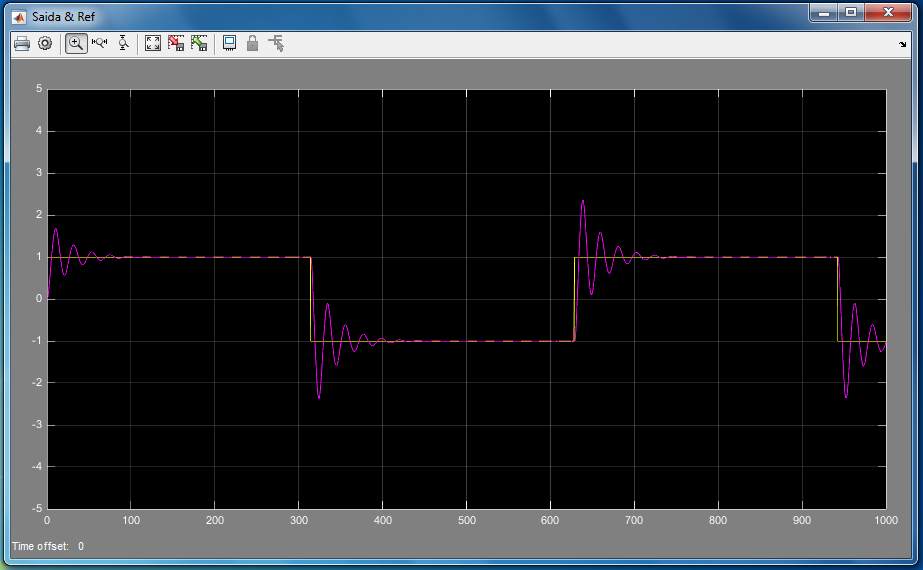
\includegraphics[scale=0.3]{Images/Mamdani_9_square.png}
  \caption{Saída obtida (a roxo) e esperada (a amarelo), utilizando a onda quadrada como referência e um controlador \emph{Mamdani} de $9$ regras}
\end{figure}

\begin{figure}[h]
  \centering
      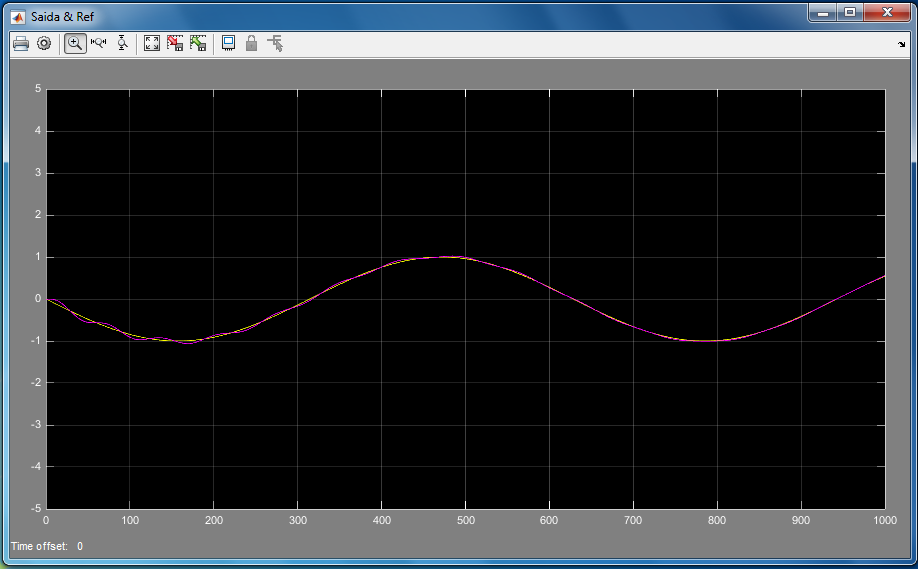
\includegraphics[scale=0.3]{Images/Mamdani_9_sin.png}
  \caption{Saída obtida (a roxo) e esperada (a amarelo), utilizando a onda quadrada como referência e um controlador \emph{Mamdani} de $9$ regras}
\end{figure}

Quando a referência mantém uma tendência mais ou menos constante, apresentando variações mais suaves, é mais fácil para o controlador corrigir eventuais erros.

De qualquer das formas, mesmo para referências quadradas, verificámos uma correta aplicação das regras dos controladores. Considerando, por exemplo, a situação seguinte:

\begin{figure}[H]
  \centering
      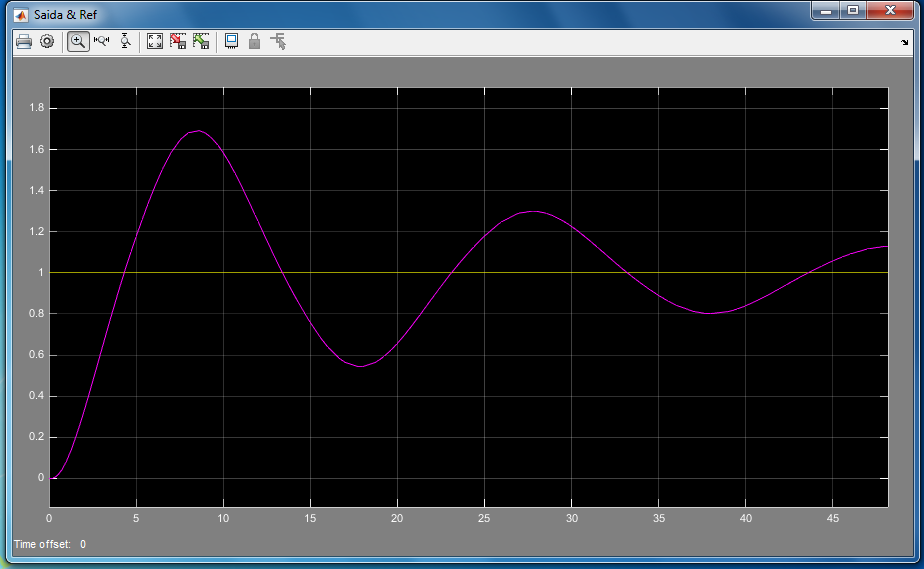
\includegraphics[scale=0.3]{Images/Mamdani_9_square_zoom.png}
  \caption{Exemplo de aplicação das regras do controlador \emph{Mamdani} de $9$ regras}
\end{figure}

Nesta situação a saída do controlador começa por ser inferior ao valor da sua referência, constituindo, portanto, um erro positivo. Uma vez que o valor da saída se está a aproximar da referência, concluímos que a sua variação é negativa (pois o erro está a diminuir, fruto da aproximação da saída à referência).

Assim, pela aplicação das regras apresentadas, o controlador não necessita de \emph{"travar"} nem \emph{"acelerar"} a saída, mantendo esta com a mesma tendência, caminhando no sentido de diminuição do erro, ou seja, no sentido da referência que pretendemos seguir.

De facto, tal situação é verificada, uma vez que o valor da saída do controlador aumenta, chegando até a igualar a referência. Nesse momento, estamos perante uma situação de erro nulo, e a sua variação é negativa (analisando os instantes imediatamente anteriores a esta situação verificamos que o erro se encontra a diminuir, o que corresponde a uma variação negativa). Assim, por aplicação das regras estudadas, o controlador deveria, nesta situação, \emph{"travar"} a saída.

Efetivamente, tal ação é realizada, mas os seus efeitos não são sentidos no imediato, uma vez que a saída do controlador continua a aumentar, afastando-se do valor da referência, até que começa a diminuir, voltando a ir ao encontro da referência que se pretende seguir.

Para além destes factos, constatámos ainda, à semelhança do que previmos anteriormente neste documento, que ao aumentarmos o número de regras do controlador, este iria ter um melhor desempenho. De facto, verificámos uma melhoria significativa desse desempenho, quer utilizando como referência a onda quadrada, quer utilizando a senoide, sendo esta percentualmente mais elevada nas situações em que a referência utilizada é a onda senoide, ou seja, o seno.

Tal como referimos anteriormente, este resultado é esperado, uma que com um maior número de regras os ajustes realizados pelo controlador podem ser mais suaves e adaptados a cada situação em particular, resultando num melhor desempenho do mesmo.

Da mesma forma, ao introduzirmos perturbações nas referências fornecidas aos controladores podemos verificar uma baixa no seu desempenho, sendo por vezes bastante significativa.

De facto, este resultado também era por nós previsto, uma vez que ao considerarmos uma perturbação na referência estamos a adulterar os sinais de entrada do controlador, o que se vai repercutir na ação por ele tomada, nem sempre tomando a melhor ação para a situação em questão. Mais ainda, quando considerámos perturbações em simultâneo no atuador e na carga o desempenho dos controladores baixou ainda mais, tal como previsto.

Gostaríamos também de referir que, de uma forma geral, os controladores do tipo \emph{Sugeno} apresentaram melhores resultados do que os \emph{Mamdani}, no entanto, estes últimos apresentam maior tolerância à presença de perturbações no atuador e na carga, uma vez que nessas situações obtiveram reduções relativas do desempenho inferiores às presenciadas pelos controladores do tipo \emph{Sugeno}.

Tendo em conta os resultados apresentamos, concluímos que, ao utilizarmos a onda senoide como referência, aliada a um controlador do tipo \emph{Sugeno} com $25$ regras, e sem considerar nenhuma perturbação da referência, conseguimos seguir da melhor forma a referência fornecida ao controlador. Esta é, portanto, a configuração que apresentou melhores resultados nos testes realizados.

De facto, analisando os testes realizados temos consciência de que seria necessário ter testado um maior número de situações, nomeadamente variando o método de desfuzificação do controlador, os operadores de conjunção/disjunção dos antecedentes, implicação e agregação das saídas.

Testando os diferentes modelos apresentados com controladores onde fossem variadas estas propriedades permitia-nos obter resultados mais conclusivos na comparação dos controladores testados. Dessa forma poderíamos até obter uma configuração que, com alguma confiança, nos permitisse concluir ser a melhor para a situação em estudo.

No entanto, como já foi anteriormente referido, não dispusemos de tempo suficiente para realizar todos os testes pretendidos, uma vez que cada teste demorou bastante tempo a ser executado nas nossas máquinas. Assim, foi-nos apenas possível realizar os testes indicados. Não obstante, este seria um aspeto que tencionaríamos melhorar em iterações futuras do trabalho.

\pagebreak

\section{Anexos}

Nesta secção apresentamos os resultados obtidos em cada teste realizado ao processo: Para além da performance registada (e que pode ser consultada na 3ª secção deste documento) registámos também a saída obtida e esperada para cada processo, a partir das quais foi calculada a sua performance.

\vspace{.2cm}

%======================Mamdani_9_square=====================================

\begin{figure}[h]
  \centering
      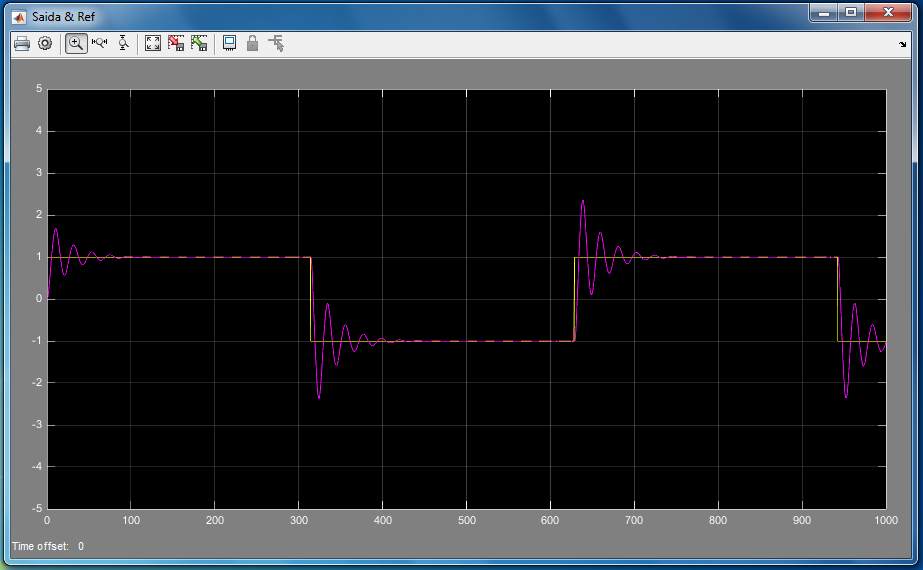
\includegraphics[scale=0.3]{Images/Mamdani_9_square.png}
  \caption{Saída obtida (a roxo) e esperada (a amarelo), utilizando a onda quadrada como referência e um controlador \emph{Mamdani} de $9$ regras}
\end{figure}

\begin{figure}[h]
  \centering
      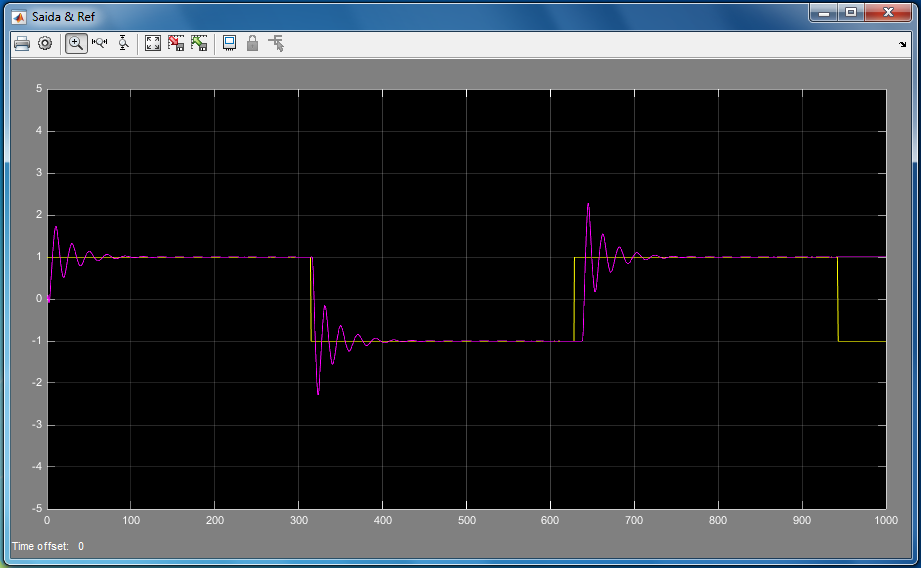
\includegraphics[scale=0.3]{Images/Mamdani_9_square_actuator.png}
  \caption{Saída obtida (a roxo) e esperada (a amarelo), utilizando a onda quadrada como referência e um controlador \emph{Mamdani} de $9$ regras, e com perturbações no atuador}
\end{figure}

\begin{figure}[h]
  \centering
      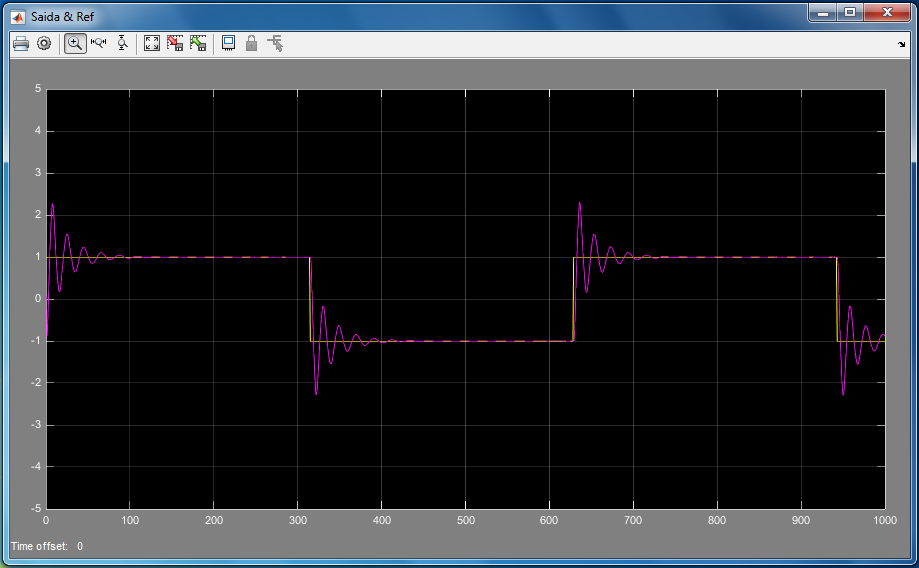
\includegraphics[scale=0.3]{Images/Mamdani_9_square_charge.png}
  \caption{Saída obtida (a roxo) e esperada (a amarelo), utilizando a onda quadrada como referência e um controlador \emph{Mamdani} de $9$ regras, e com perturbações na carga}
\end{figure}


\begin{figure}[h]
  \centering
      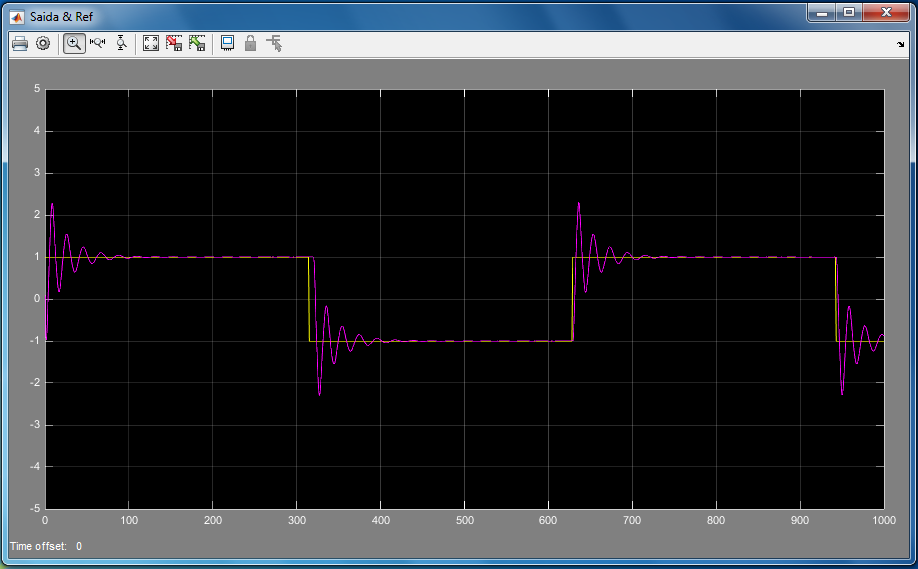
\includegraphics[scale=0.3]{Images/Mamdani_9_square_actuator_charge.png}
  \caption{Saída obtida (a roxo) e esperada (a amarelo), utilizando a onda quadrada como referência e um controlador \emph{Mamdani} de $9$ regras, e com perturbações no atuador e na carga}
\end{figure}

%======================Mamdani_9_sin========================================

\begin{figure}[h]
  \centering
      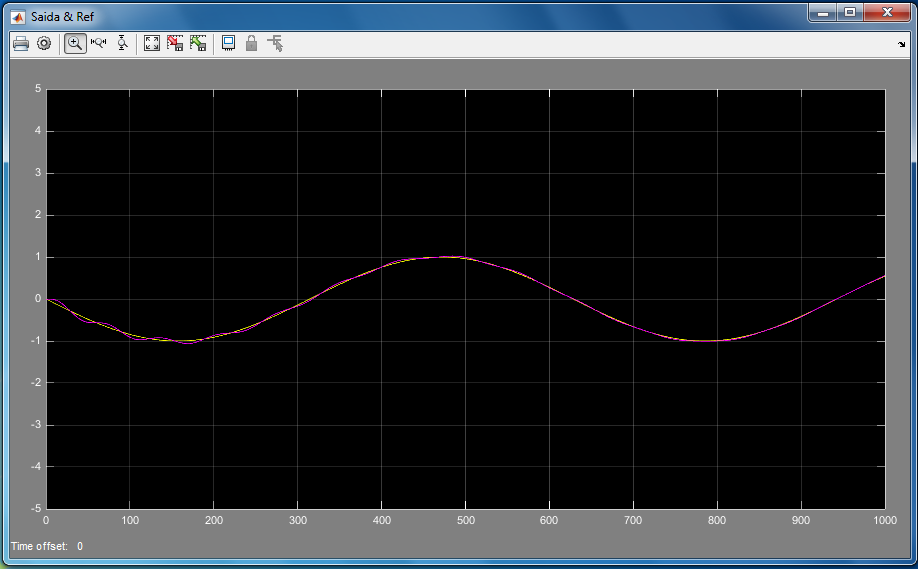
\includegraphics[scale=0.3]{Images/Mamdani_9_sin.png}
  \caption{Saída obtida (a roxo) e esperada (a amarelo), utilizando a onda senoide (seno) como referência e um controlador \emph{Mamdani} de $9$ regras}
\end{figure}

\begin{figure}[h]
  \centering
      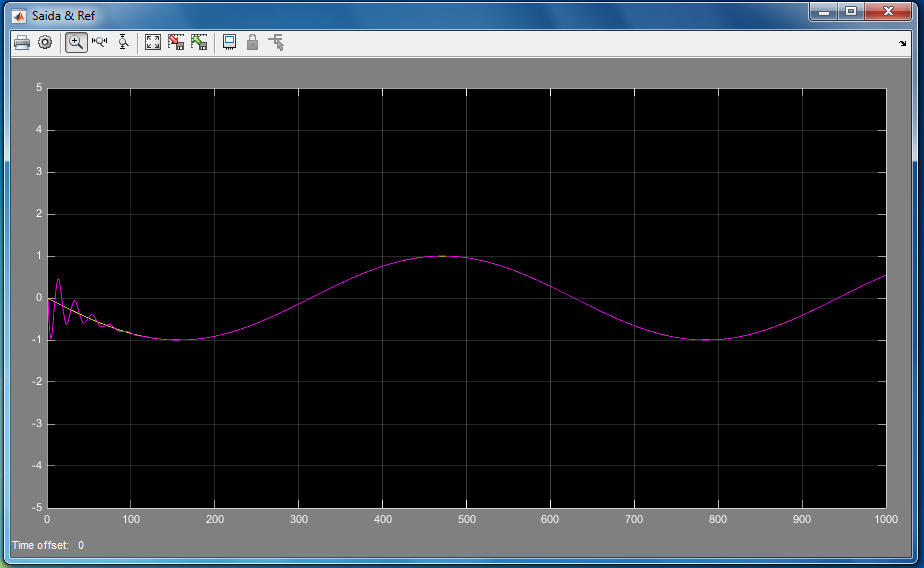
\includegraphics[scale=0.3]{Images/Mamdani_9_sin_actuator.png}
  \caption{Saída obtida (a roxo) e esperada (a amarelo), utilizando a onda senoide (seno) como referência e um controlador \emph{Mamdani} de $9$ regras, e com perturbações no atuador}
\end{figure}

\begin{figure}[h]
  \centering
      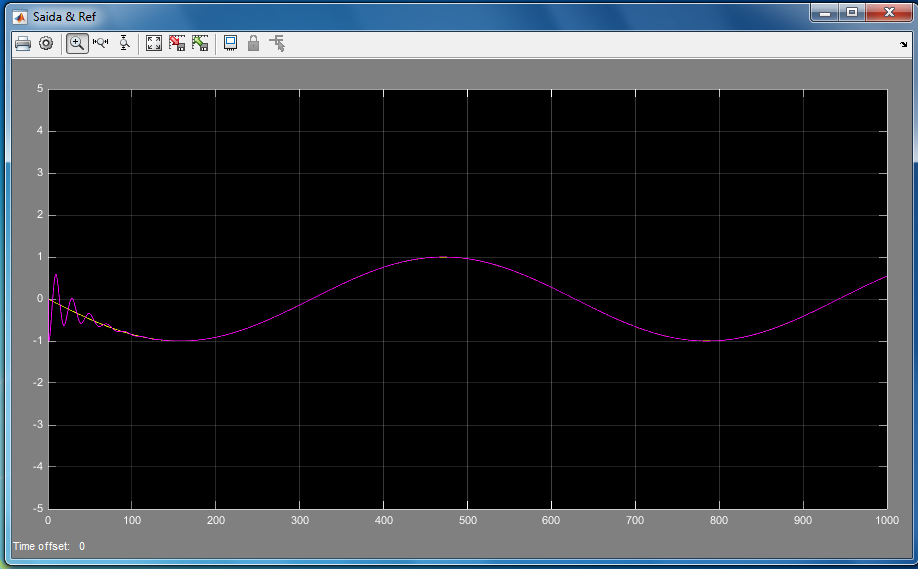
\includegraphics[scale=0.3]{Images/Mamdani_9_sin_charge.png}
  \caption{Saída obtida (a roxo) e esperada (a amarelo), utilizando a onda senoide (seno) como referência e um controlador \emph{Mamdani} de $9$ regras, e com perturbações na carga}
\end{figure}

\begin{figure}[h]
  \centering
      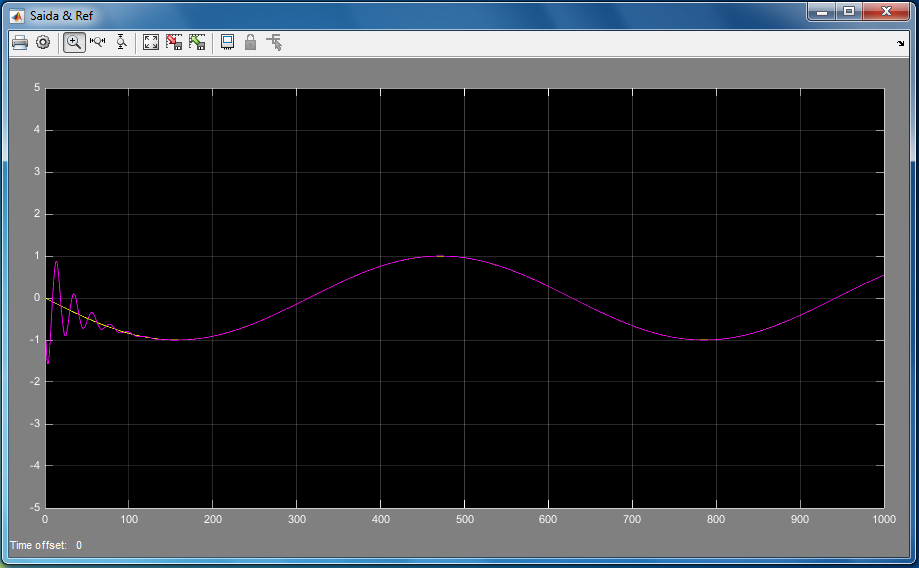
\includegraphics[scale=0.3]{Images/Mamdani_9_sin_actuator_charge.png}
  \caption{Saída obtida (a roxo) e esperada (a amarelo), utilizando a onda senoide (seno) como referência e um controlador \emph{Mamdani} de $9$ regras, e com perturbações no atuador e na carga}
\end{figure}

%======================Mamdani_25_square====================================

\begin{figure}[h]
  \centering
      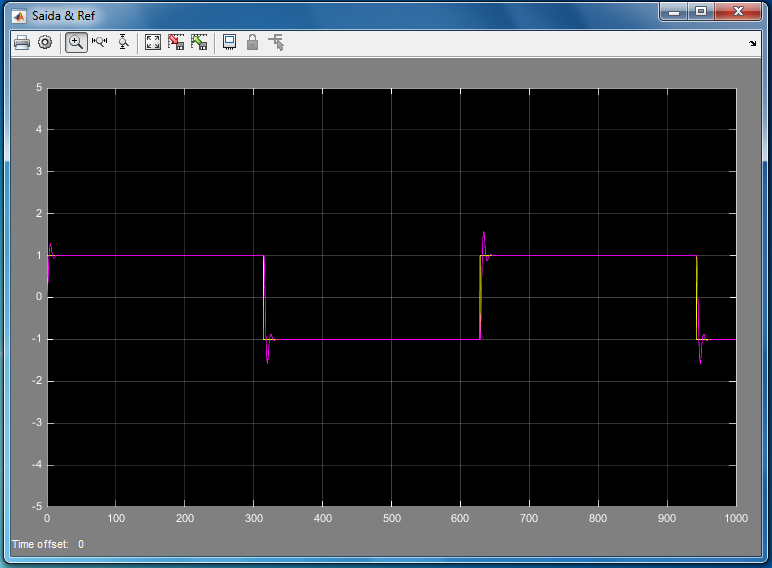
\includegraphics[scale=0.3]{Images/Mamdani_25_square.png}
  \caption{Saída obtida (a roxo) e esperada (a amarelo), utilizando a onda quadrada como referência e um controlador \emph{Mamdani} de $25$ regras}
\end{figure}

\begin{figure}[h]
  \centering
      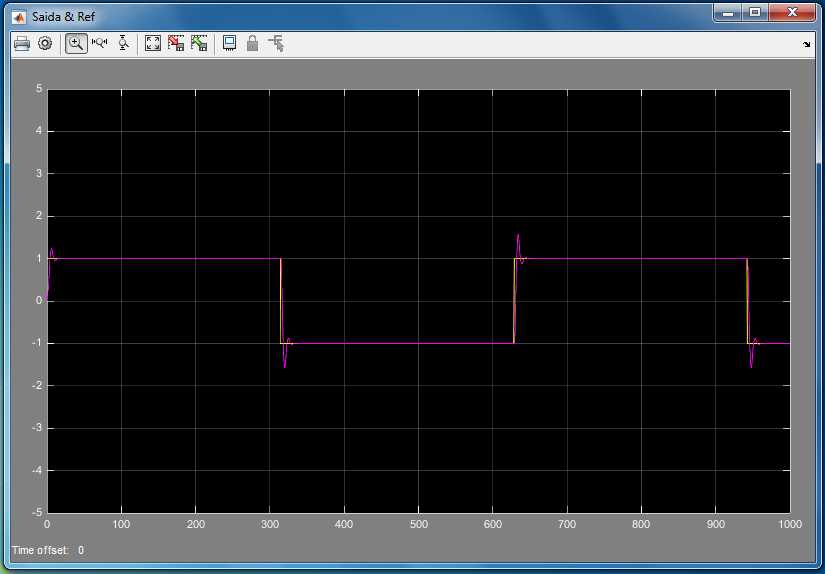
\includegraphics[scale=0.3]{Images/Mamdani_25_square_actuator.png}
  \caption{Saída obtida (a roxo) e esperada (a amarelo), utilizando a onda quadrada como referência e um controlador \emph{Mamdani} de $25$ regras, e com perturbações no atuador}
\end{figure}

\begin{figure}[h]
  \centering
      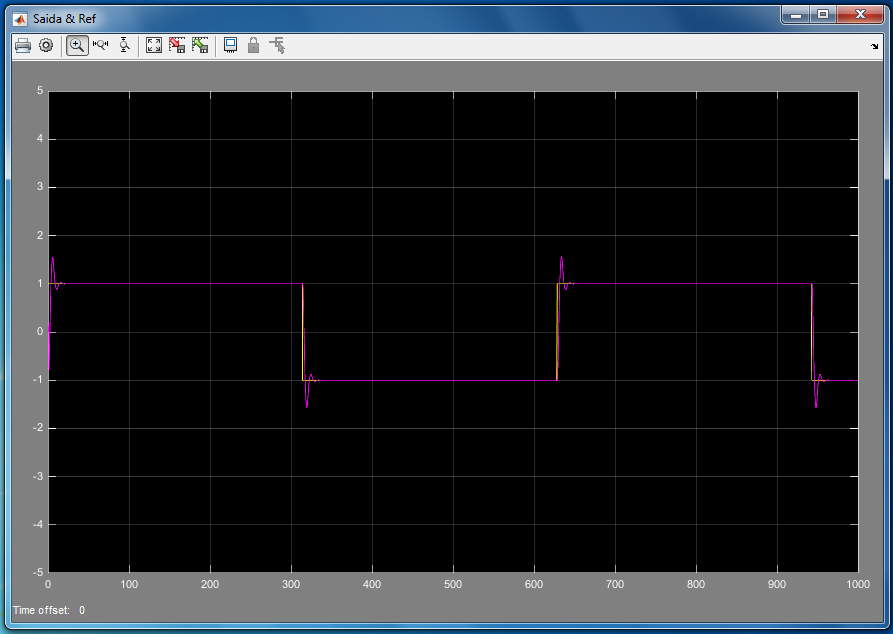
\includegraphics[scale=0.3]{Images/Mamdani_25_square_charge.png}
  \caption{Saída obtida (a roxo) e esperada (a amarelo), utilizando a onda quadrada como referência e um controlador \emph{Mamdani} de $25$ regras, e com perturbações na carga}
\end{figure}

\begin{figure}[h]
  \centering
      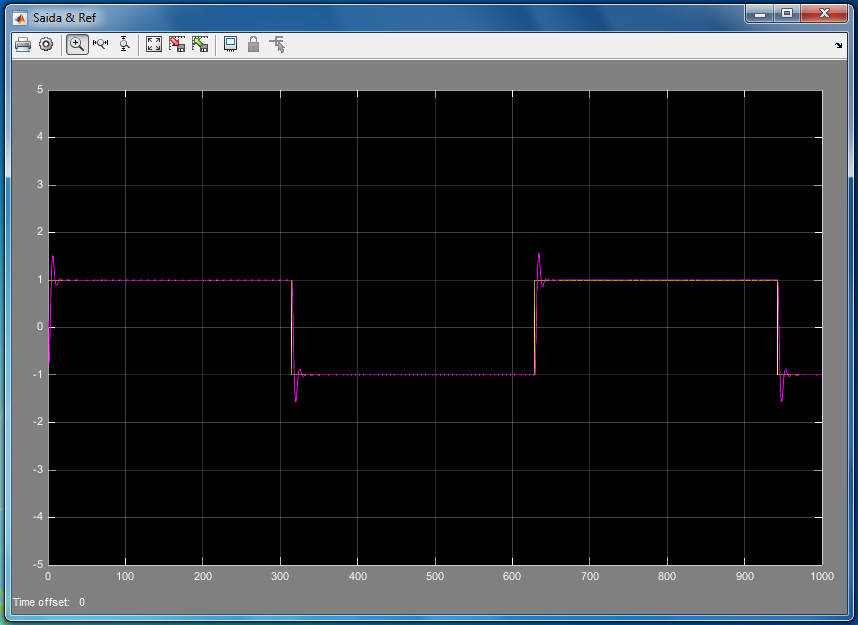
\includegraphics[scale=0.3]{Images/Mamdani_25_square_actuator_charge.png}
  \caption{Saída obtida (a roxo) e esperada (a amarelo), utilizando a onda quadrada como referência e um controlador \emph{Mamdani} de $25$ regras, e com perturbações no atuador e na carga}
\end{figure}

%======================Mamdani_25_sin=======================================

\begin{figure}[h]
  \centering
      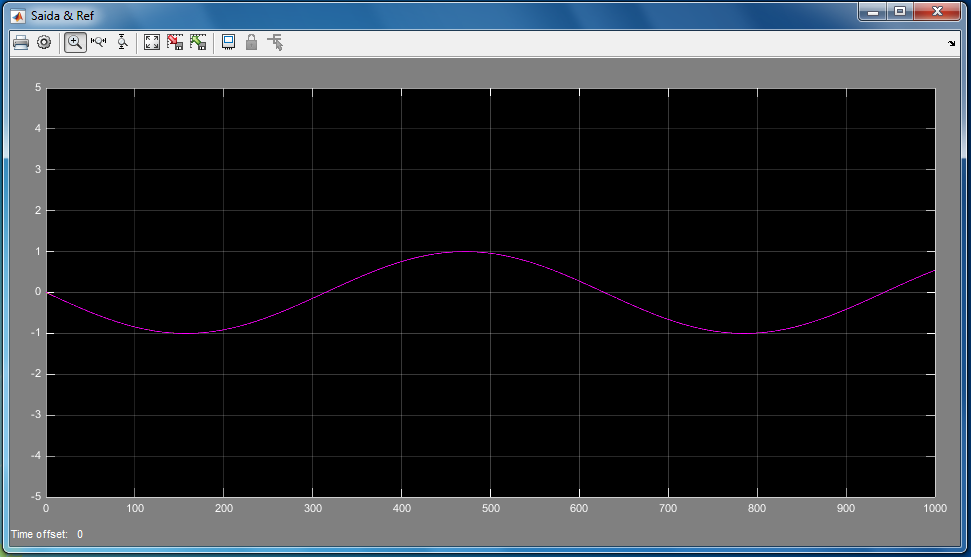
\includegraphics[scale=0.3]{Images/Mamdani_25_sin.png}
  \caption{Saída obtida (a roxo) e esperada (a amarelo), utilizando a onda senoide (seno) como referência e um controlador \emph{Mamdani} de $25$ regras}
\end{figure}

\begin{figure}[h]
  \centering
      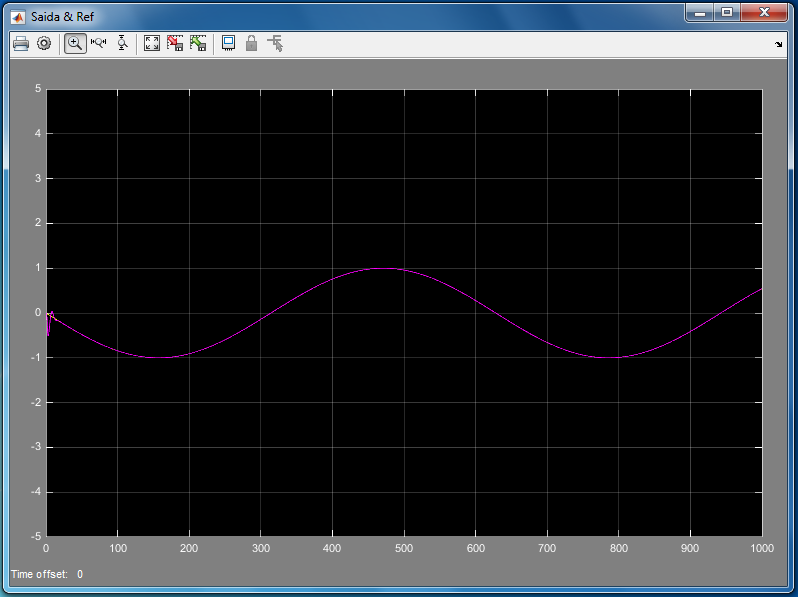
\includegraphics[scale=0.3]{Images/Mamdani_25_sin_actuator.png}
  \caption{Saída obtida (a roxo) e esperada (a amarelo), utilizando a onda senoide (seno) como referência e um controlador \emph{Mamdani} de $25$ regras, e com perturbações no atuador}
\end{figure}

\begin{figure}[h]
  \centering
      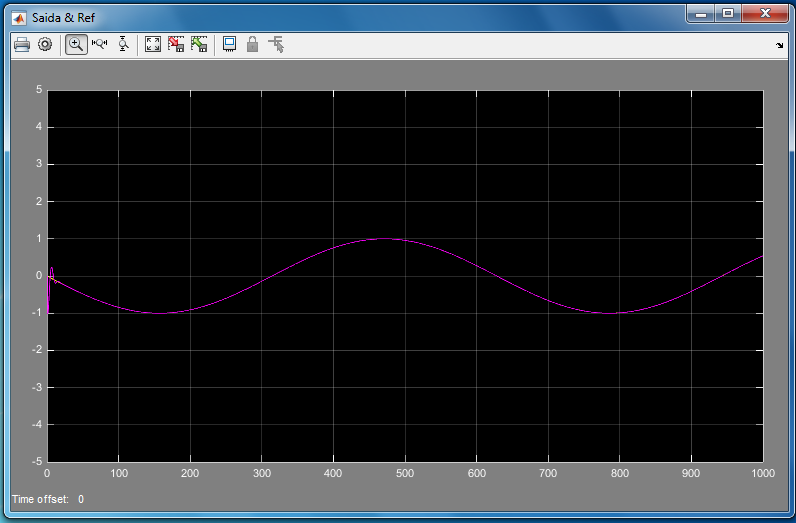
\includegraphics[scale=0.3]{Images/Mamdani_25_sin_charge.png}
  \caption{Saída obtida (a roxo) e esperada (a amarelo), utilizando a onda senoide (seno) como referência e um controlador \emph{Mamdani} de $25$ regras, e com perturbações na carga}
\end{figure}

\begin{figure}[h]
  \centering
      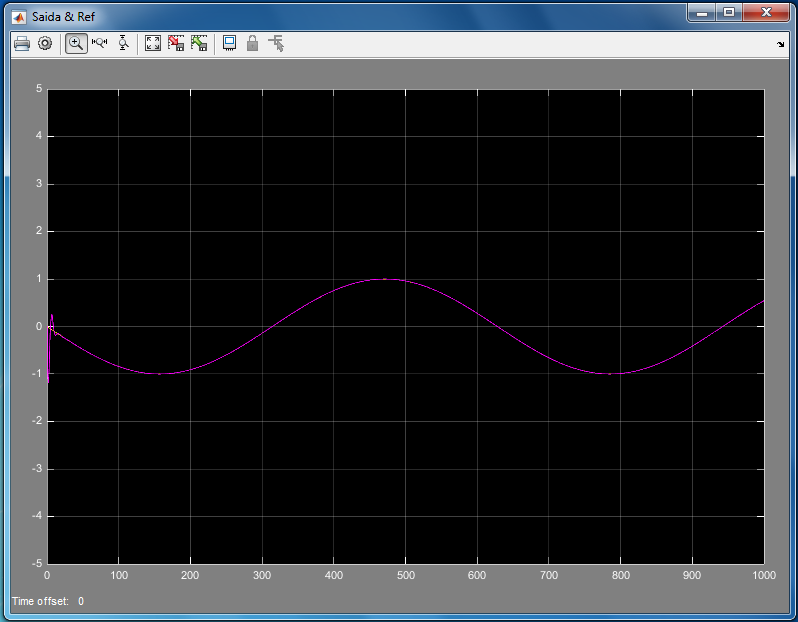
\includegraphics[scale=0.3]{Images/Mamdani_25_sin_actuator_charge.png}
  \caption{Saída obtida (a roxo) e esperada (a amarelo), utilizando a onda senoide (seno) como referência e um controlador \emph{Mamdani} de $25$ regras, e com perturbações no atuador e na carga}
\end{figure}

\clearpage

%======================Sugeno_9_square======================================

\begin{figure}[h]
  \centering
      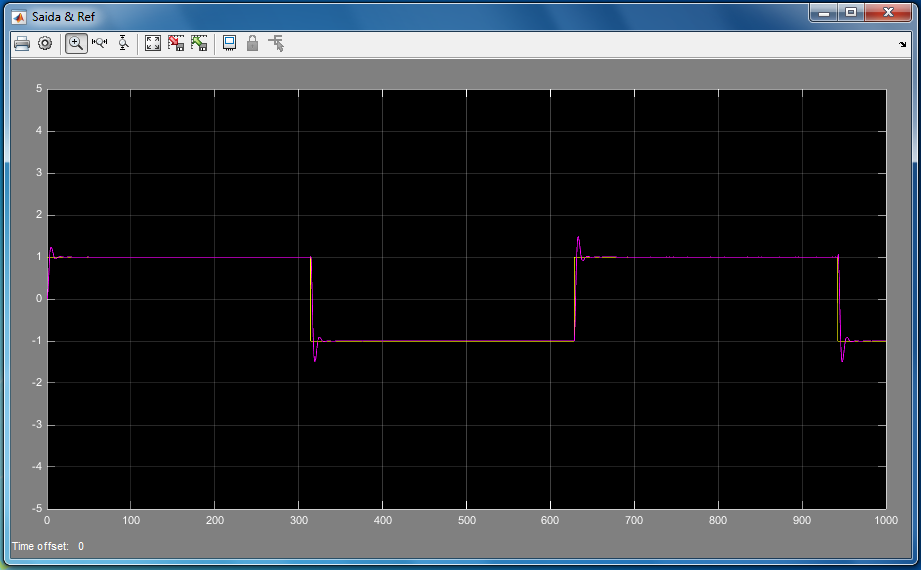
\includegraphics[scale=0.3]{Images/Sugeno_9_square.png}
  \caption{Saída obtida (a roxo) e esperada (a amarelo), utilizando a onda quadrada como referência e um controlador \emph{Sugeno} de $9$ regras}
\end{figure}

\begin{figure}[h]
  \centering
      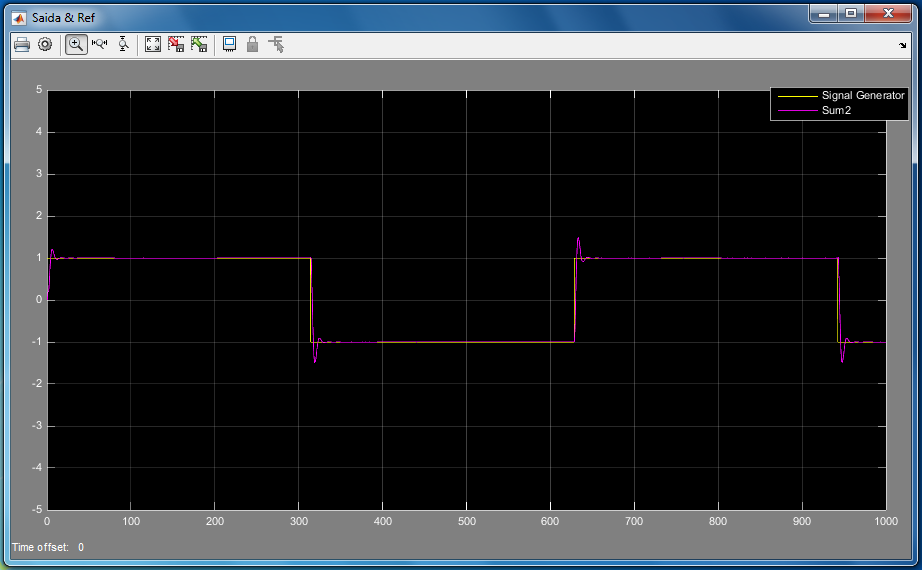
\includegraphics[scale=0.3]{Images/Sugeno_9_square_actuator.png}
  \caption{Saída obtida (a roxo) e esperada (a amarelo), utilizando a onda quadrada como referência e um controlador \emph{Sugeno} de $9$ regras, e com perturbações no atuador}
\end{figure}

\begin{figure}[h]
  \centering
      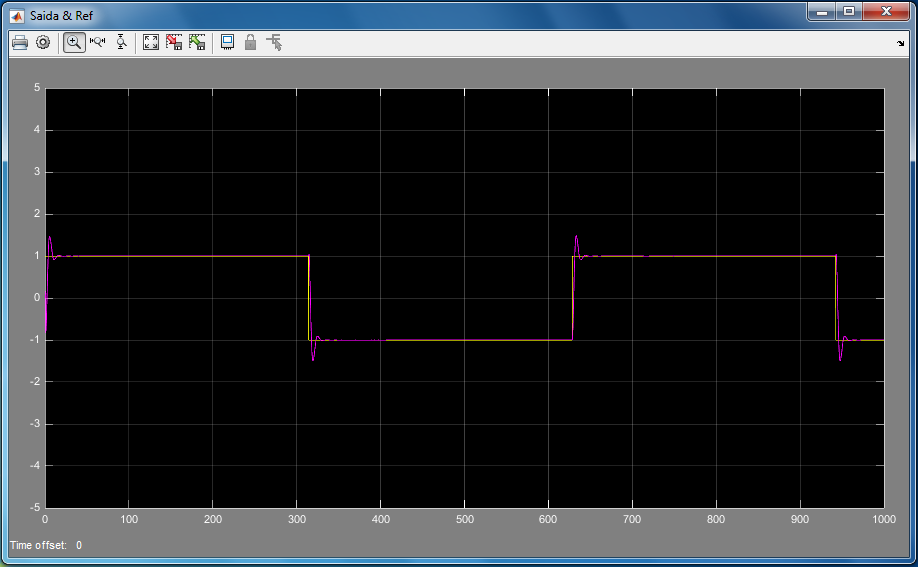
\includegraphics[scale=0.3]{Images/Sugeno_9_square_charge.png}
  \caption{Saída obtida (a roxo) e esperada (a amarelo), utilizando a onda quadrada como referência e um controlador \emph{Sugeno} de $9$ regras, e com perturbações na carga}
\end{figure}

\begin{figure}[h]
  \centering
      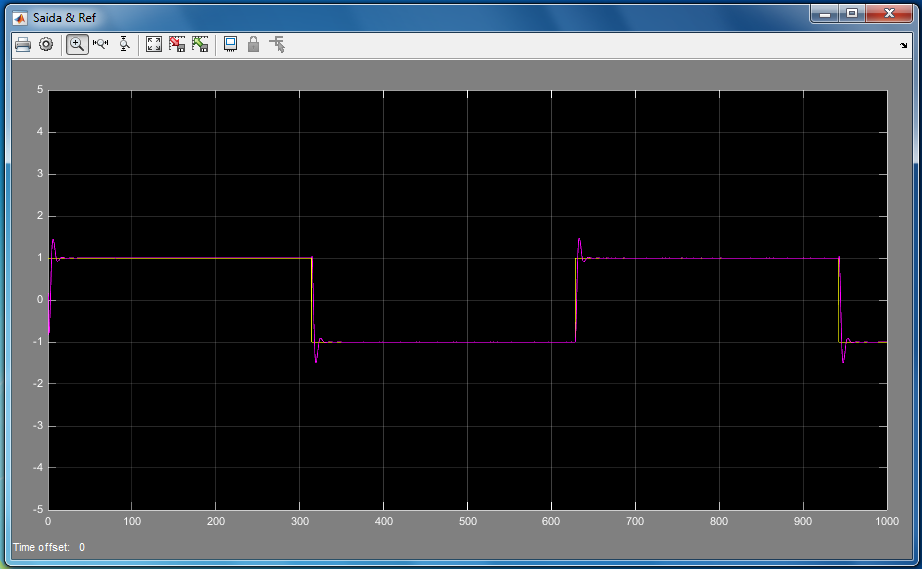
\includegraphics[scale=0.3]{Images/Sugeno_9_square_actuator_charge.png}
  \caption{Saída obtida (a roxo) e esperada (a amarelo), utilizando a onda quadrada como referência e um controlador \emph{Sugeno} de $9$ regras, e com perturbações no atuador e na carga}
\end{figure}

\clearpage

%======================Sugeno_9_sin=========================================

\begin{figure}[h]
  \centering
      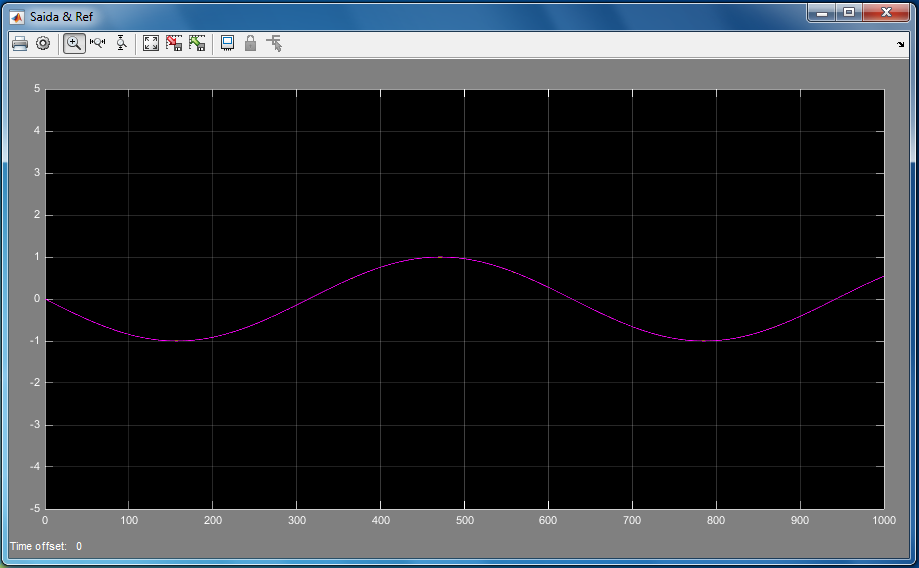
\includegraphics[scale=0.3]{Images/Sugeno_9_sin.png}
  \caption{Saída obtida (a roxo) e esperada (a amarelo), utilizando a onda senoide (seno) como referência e um controlador \emph{Sugeno} de $9$ regras}
\end{figure}

\begin{figure}[h]
  \centering
      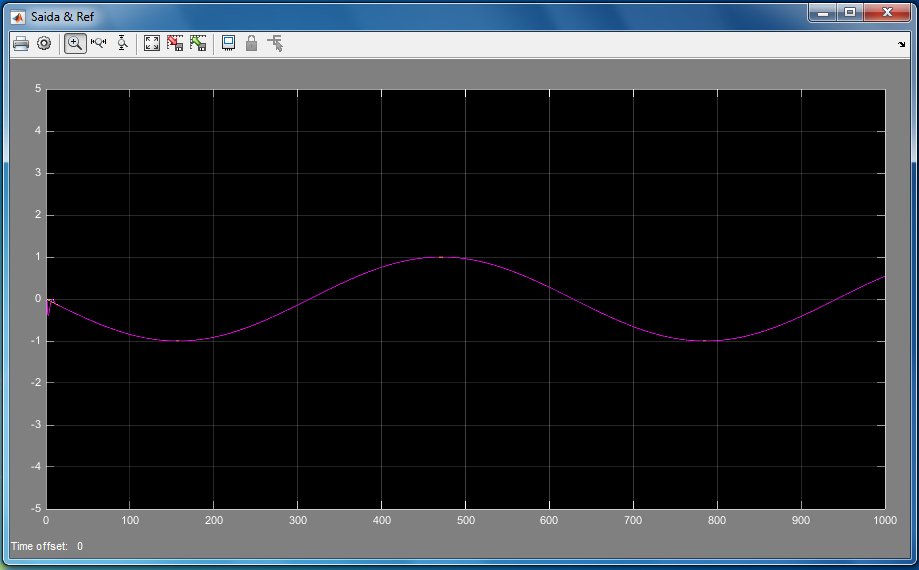
\includegraphics[scale=0.3]{Images/Sugeno_9_sin_actuator.png}
  \caption{Saída obtida (a roxo) e esperada (a amarelo), utilizando a onda senoide (seno) como referência e um controlador \emph{Sugeno} de $9$ regras, e com perturbações no atuador}
\end{figure}

\begin{figure}[h]
  \centering
      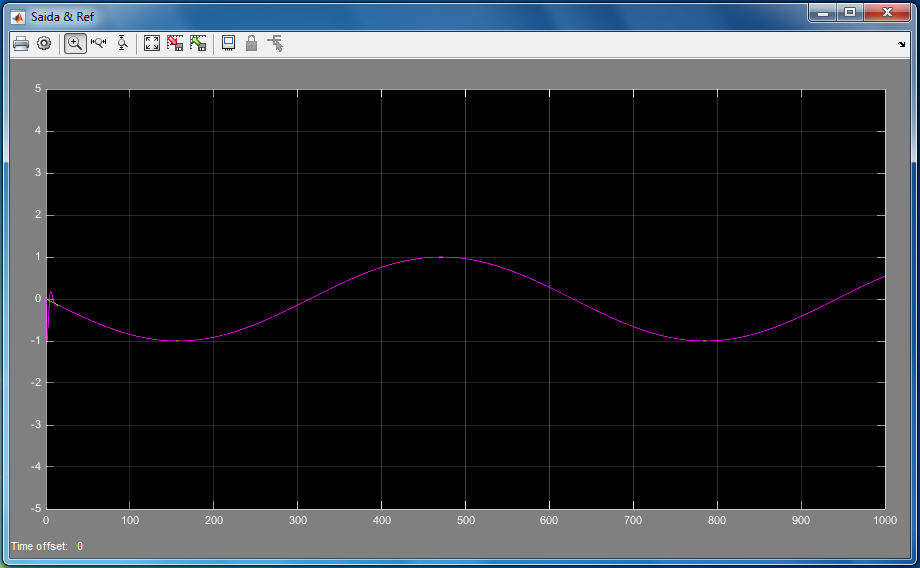
\includegraphics[scale=0.3]{Images/Sugeno_9_sin_charge.png}
  \caption{Saída obtida (a roxo) e esperada (a amarelo), utilizando a onda senoide (seno) como referência e um controlador \emph{Sugeno} de $9$ regras, e com perturbações na carga}
\end{figure}

\begin{figure}[h]
  \centering
      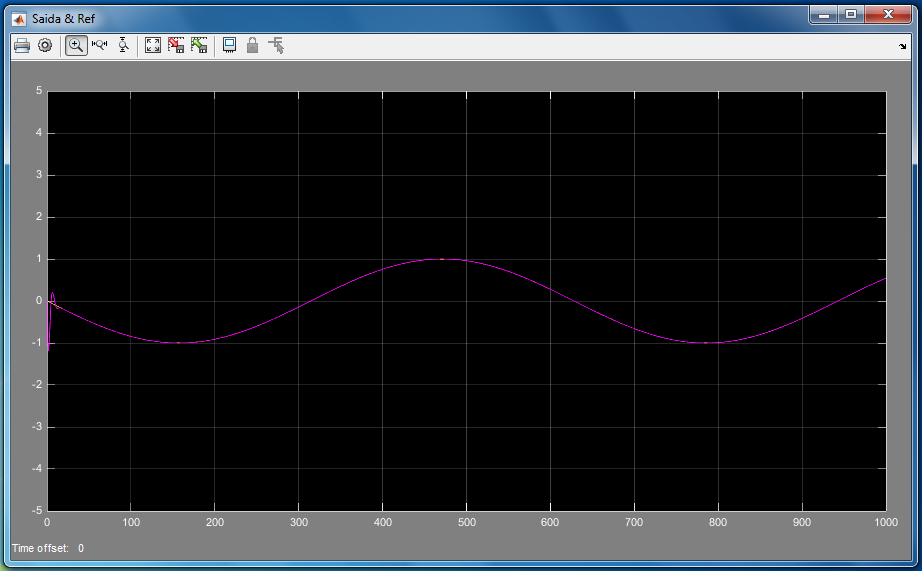
\includegraphics[scale=0.3]{Images/Sugeno_9_sin_actuator_charge.png}
  \caption{Saída obtida (a roxo) e esperada (a amarelo), utilizando a onda senoide (seno) como referência e um controlador \emph{Sugeno} de $9$ regras, e com perturbações no atuador e na carga}
\end{figure}

%======================Sugeno_25_square=====================================

\begin{figure}[h]
  \centering
      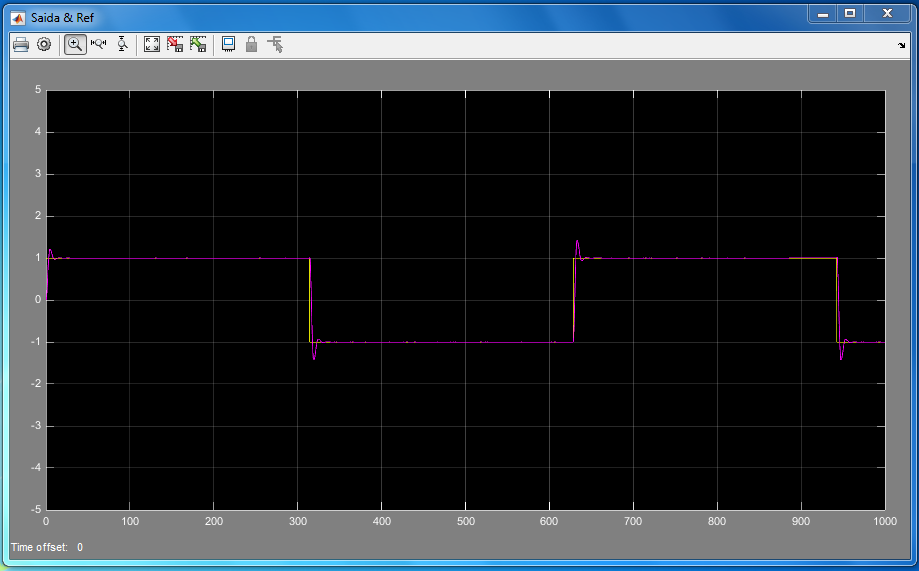
\includegraphics[scale=0.3]{Images/Sugeno_25_square.png}
  \caption{Saída obtida (a roxo) e esperada (a amarelo), utilizando a onda quadrada como referência e um controlador \emph{Sugeno} de $25$ regras}
\end{figure}

\begin{figure}[h]
  \centering
      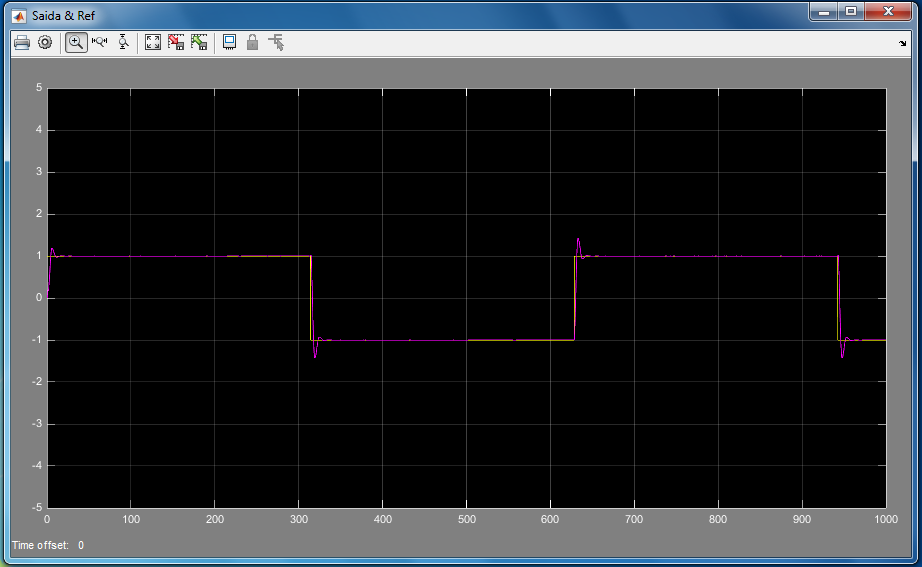
\includegraphics[scale=0.3]{Images/Sugeno_25_square_actuator.png}
  \caption{Saída obtida (a roxo) e esperada (a amarelo), utilizando a onda quadrada como referência e um controlador \emph{Sugeno} de $25$ regras, e com perturbações no atuador}
\end{figure}

\begin{figure}[h]
  \centering
      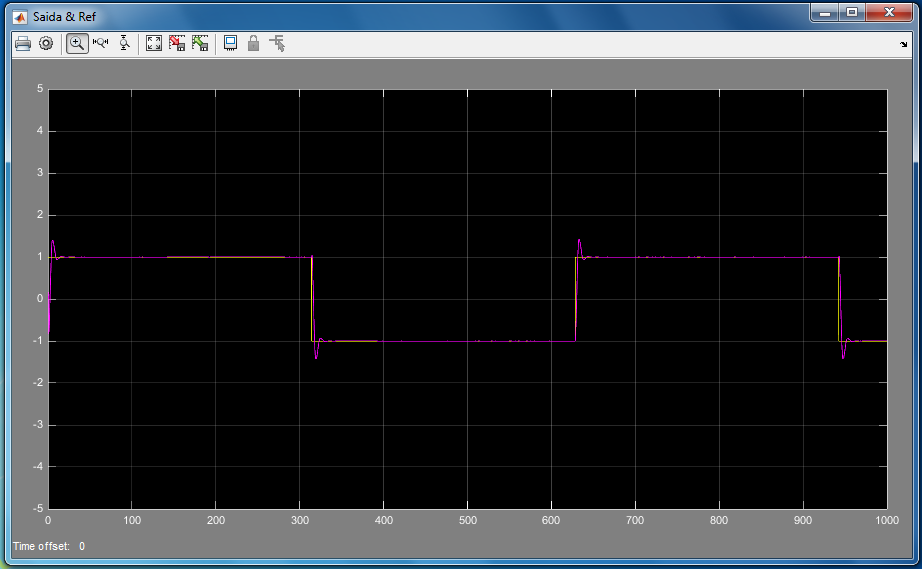
\includegraphics[scale=0.3]{Images/Sugeno_25_square_charge.png}
  \caption{Saída obtida (a roxo) e esperada (a amarelo), utilizando a onda quadrada como referência e um controlador \emph{Sugeno} de $9$ regras, e com perturbações na carga}
\end{figure}

\begin{figure}[h]
  \centering
      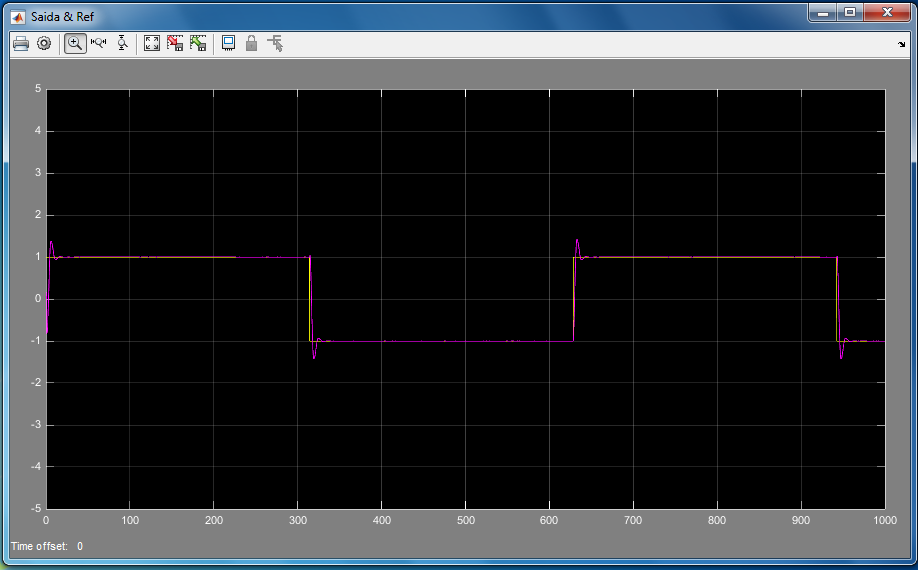
\includegraphics[scale=0.3]{Images/Sugeno_25_square_actuator_charge.png}
  \caption{Saída obtida (a roxo) e esperada (a amarelo), utilizando a onda quadrada como referência e um controlador \emph{Sugeno} de $25$ regras, e com perturbações no atuador e na carga}
\end{figure}

%======================Sugeno_25_sin========================================

\begin{figure}[h]
  \centering
      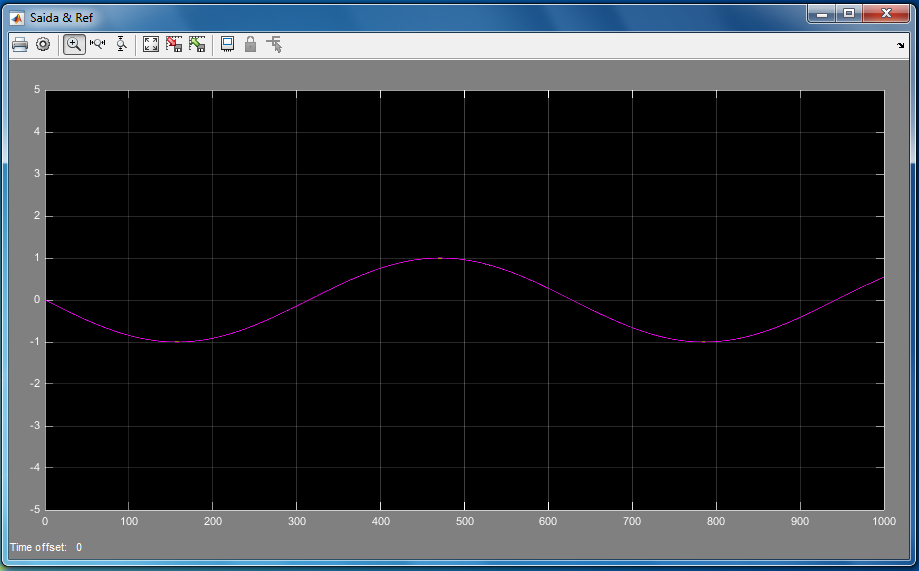
\includegraphics[scale=0.3]{Images/Sugeno_25_sin.png}
  \caption{Saída obtida (a roxo) e esperada (a amarelo), utilizando a onda senoide (seno) como referência e um controlador \emph{Sugeno} de $25$ regras}
\end{figure}

\begin{figure}[h]
  \centering
      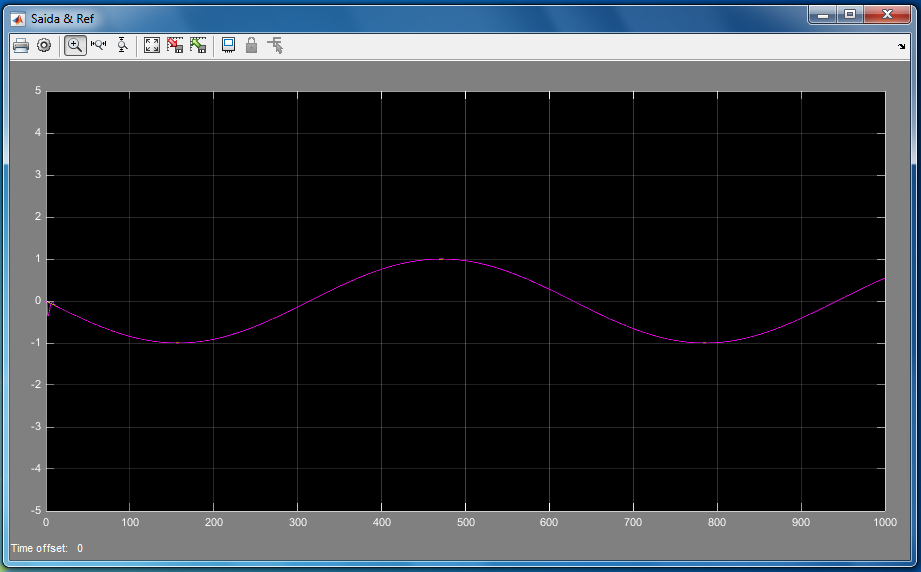
\includegraphics[scale=0.3]{Images/Sugeno_25_sin_actuator.png}
  \caption{Saída obtida (a roxo) e esperada (a amarelo), utilizando a onda senoide (seno) como referência e um controlador \emph{Sugeno} de $25$ regras, e com perturbações no atuador}
\end{figure}

\begin{figure}[h]
  \centering
      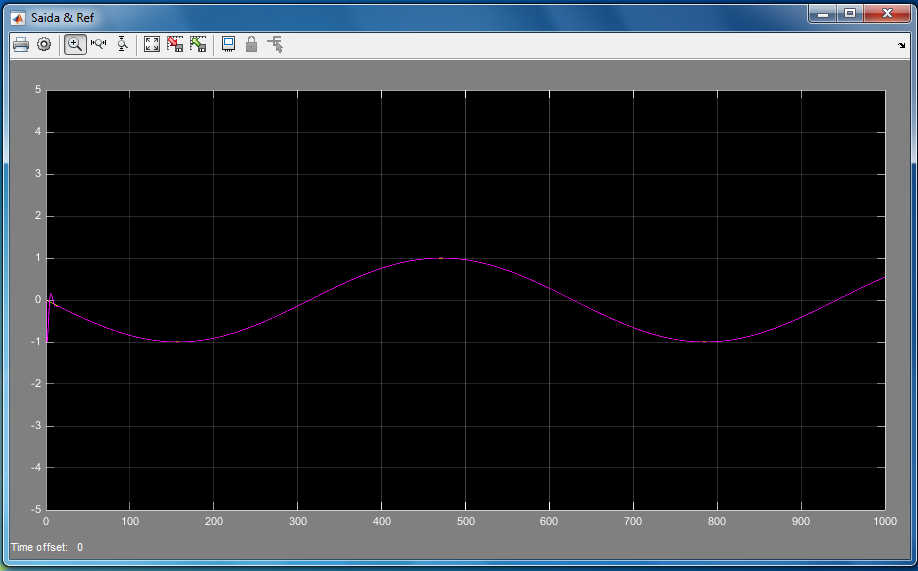
\includegraphics[scale=0.3]{Images/Sugeno_25_sin_charge.png}
  \caption{Saída obtida (a roxo) e esperada (a amarelo), utilizando a onda senoide (seno) como referência e um controlador \emph{Sugeno} de $25$ regras, e com perturbações na carga}
\end{figure}

\begin{figure}[h]
  \centering
      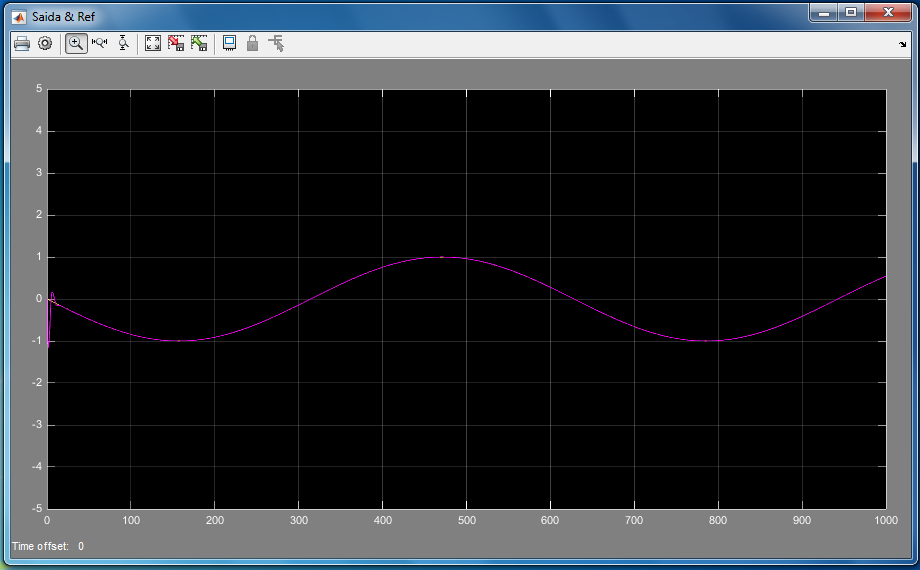
\includegraphics[scale=0.3]{Images/Sugeno_25_sin_actuator_charge.png}
  \caption{Saída obtida (a roxo) e esperada (a amarelo), utilizando a onda senoide (seno) como referência e um controlador \emph{Sugeno} de $25$ regras, e com perturbações no atuador e na carga}
\end{figure}

\end{document}